\documentclass[11pt]{article}

%\usepackage{fullpage} % this changes margins
\usepackage[margin=1in]{geometry}  % change the margin size 
\usepackage{amsfonts, amsmath, amssymb} % for the math 
\usepackage{graphicx}   % for the graphic 
\usepackage[none]{hyphenat} %prevent latex from using hyphenated words
\usepackage{fancyhdr} % allow to create custom fancy header and footer  
\usepackage{float}
\usepackage[nottoc,notlot,notlof]{tocbibind} % package for table of content


\pagestyle{fancy}
\fancyhead{} % use the default header
\fancyfoot{} % use the default footer
\fancyhead[L]{\slshape \MakeUppercase{Place Title Here}} % L for left
\fancyhead[R]{\slshape Student Name} % R for right 
\fancyfoot[C]{\thepage} % c for center 
% \renewcommand{\headrulewidth}{0pt} % remove the horizontal line(the thickness of the line is 0)
% \renewcommand{\footrulewidth}{0pt}   % remove the foot underline 

\parindent 0ex % disable the paragraph indent 
%\setlength{\parindent}{4em} % change the width of the indent 
% \setlength{\parskip}{1em} % change the width of the paragraph skip 	 	
\renewcommand{\baselinestretch}{1.5} % set the line spacing of paragraph 


\def\eq1{Y=\frac{x}{3x^2+7}}
\def\labelaxes{Remember to include a scale and label your axes.}

\begin{document}	
% add the title page
\begin{titlepage}
\begin{center}
\vspace*{1cm}  % add move space
\Large{\textbf{IB Mathematics SL}}\\
\Large{\textbf{Internal Assessment}}\\
\vfill  % vertical fill:  this will automatically adjust the space between two elements
		

\line(1,0){400}\\ [1mm] % create a herizontall line  with width 400
% [1mm] means add 1mm space between two elements

\huge{\textbf{This is a Sample Title  \LaTeX }} \\ [3mm]
\Large{\textbf{- This is a Sample Subtitle -}}\\ [1mm]
\line(1,0){400}
\vfill
By Student Name\\
Student ID \\
\today % set today's date

\end{center}
\end{titlepage}


\tableofcontents
\thispagestyle{empty} % delete the page style for this page
\clearpage % not count this page number



\setcounter{page}{1} % set the page number 1

\title{My Practice \LaTeX \  Document}
\author{Arthur Feng}
\date{\today}
\maketitle 

\section{Introduction}

Some text: "Sometimes after I write a review people will e-mail me and ask\cite{DBHS1}, in so many words, "Never mind the overview, why would I use this distribution over another one?" In Manjaro's case this is an easy question to answer as the distribution does a lot of things well. Manjaro is a rolling release, cutting edge distribution so the project consistently provides the latest and greatest open source software. Apart from the programs in the distribution's repositories, people running Manjaro can also make use of AUR (the large collection of software submitted by Arch Linux users). This provides Manjaro users with a huge collection of packages, most of them consistently kept up to date with upstream\footnote{An example footnote} sources.\\

I found Manjaro's Xfce edition to be very fast and unusually light on memory. The distribution worked smoothly and worked well with both my physical hardware and my virtual environment. I also enjoyed Manjaro's habit of telling me when new software (particularly new versions of the Linux kernel) was available. I fumbled a little with Manjaro's settings panel and finding some settings, but in the end I was pleased with the range of configuration I could achieve with the distribution. I especially like that Manjaro makes it easy to block notifications and keep windows from stealing focus. The distribution can be made to stay pleasantly out of the way. In short, I think Manjaro is the ideal distribution for people who like the simple, cutting edge philosophy of Arch Linux, but who would like to set up the operating system with a couple of clicks and have settings adjustable through a friendly point-n-click interface. Manjaro has most of the same capabilities of Arch, but with a friendly wrapper which makes installing and working with software packages a quick, click-and-done process.

The one serious issue I ran into during my trial came in the wake of an update. After several days of smooth use I ran into a problem when, after an update, Manjaro Linux would no longer boot. Attempts at booting in fallback mode or with various kernel parameters failed to get the system to a stage where I could login. Sadly, this signaled an end to my trial and acted as a reminder of the risks in maintaining a rolling release distribution.



\section{Macros}
Graph $\eq1$. this is define before the beginning of the dcuments, which is called macros.\\
Identify the asymptotes for the graph of $\eq1$.

This is another macros: \textbf{\labelaxes}

\section{Math}
This is the beginning of the article.\\ This is from another line. 

we can also start a new paragraph by insert extra new line. 

Let's show some in line math symbol, x + 1 is trade as text. but $x + 1$ is trade as math symbol, you could see the different between two symbols. Another example is $$A = x^2 + 2x + 1 $$ represent the area of the rectangle. Then, there are more math operators:
	\subsection{superscripts}
superscripts:
$$2x^3 $$
$$2x^34 $$
$$2x^{3x + 4} $$
$$2x^{3^m + 4x + 5} $$
	\subsection{subscripts}
Same as subscripts:
$$x_1 $$
$$x_{12}$$
$$x_{y_{3m +n}} $$
	\subsection{trig, log and square}
Trig functions:
$$\sin{n} $$
$$y = \cos{m} $$

Log functions:
$$\log{m} $$
$$\log_5{m} $$
$$\ln{m} $$

Square functions:
$$\sqrt{m}$$
$$\sqrt[n]{m} $$
$$\sqrt[1 + \sqrt{x+1}]{m+n}$$
	\subsection{Fractions}
About 2/3 of the glass is full. We can also write it like $2/3$ and $\frac{2}{3}$ We can reformat the fractions like $\displaystyle{\frac{2}{3}}$, this one is much bigger. We can write more complicate equations like $$\frac{x}{x^2+4x+1}$$ as well as : $$\frac{\sqrt[n]{m}}{x^3+7y+m}$$we can also add a fraction within a fraction:$$\frac{n}{\frac{q+p}{a+b+c} + x^2}$$

\section{symbol}
The set of Natural numbers is denoted by $\mathbb{N}$. \\
There are many other symbols, such as $\mathbb{Z}$ for integer, and $\mathbb{R}$ for real number.

$\pi$
$\zeta$
$\eta$
$\equiv$

	\subsection{Function}
The function $\displaystyle{f(x)=(x-3)^x+\frac{1}{2}}$ has domain $\mathrm{D}_f:(-\infty,\infty)$ and range $\mathrm{R}_f:\left[\frac{1}{2},\infty\right)$
% \mathrm{} will remove the style of the content

$$\lim \limits_{x \to a^-}f(x)$$\\

$$\displaystyle{\lim \limits_{x \to a}\frac{f(x)-f(a)}{x-a}=f'(a)}$$\\

$$\displaystyle{\int \sin x\, dx }$$\\
% add a space between equation by  \, 

$$\displaystyle{\int_a^b}$$\\

$$\displaystyle{\int \limits_a^b}$$\\

$$\displaystyle{\int \limits_{2a}^{a+b} x^2\,dx } =  \left[ \frac{x^3}{3} \right]_a^b$$\\

$$\displaystyle{\sum \limits_{n=1}^{\infty}ar^n = a+ar+ar^2+\cdots+ ar^n}$$\\

$$\displaystyle{\int_a^b f(x) \,dx =\lim \limits_{x \to \infty} \sum \limits_{k=1}^n f(x_k) \cdot \Delta x}$$\\

$$\vec{v} = v_1 \vec{i} + v_2 \vec{j} =\langle\\ v_1,v_2\rangle$$\\



	\subsection{Parentheses}
Parentheses:
$$(x+1)$$
$$[x+1]$$
$$\{x+1\}$$
$$\$12.55$$ 
$$3\left(\frac{3}{5}\right)$$ 
$$3\left[\frac{3}{5}\right]$$ 
$$3\left\{\frac{3}{5}\right\}$$ 
$$\left|\frac{x}{x+1}\right|$$

\section{Table and Array}
The one serious issue I ran into during my trial came in the wake of an update. After several days of smooth use I ran into a problem when, after an update, Manjaro Linux would no longer boot. Attempts at booting in fallback mode or with various kernel parameters failed to get the system to a stage where I could login. Sadly, this signaled an end to my trial and acted as a reminder of the risks in maintaining a rolling release distribution(see talbe \ref{tab:table1}). \\

\begin{table}[H] % H means 	set the figure between the text.
	\centering
		\begin{tabular}{|c|c|c|c|c|c|} \hline
		$1$ & 1 &  2 & 3 & 4 & 5 \\ \hline 
		$f(x)$ &10 & 11 & 12 & 13 & 14 \\ \hline
		\end{tabular}
	\caption{Caption goes here}
	\label{tab:table1}
\end{table}


The one serious issue I ran into during my trial came in the wake of an update. After several days of smooth use I ran into a problem when, after an update, Manjaro Linux would no longer boot. Attempts at booting in fallback mode or with various kernel parameters failed to get the system to a stage where I could login. Sadly, this signaled an end to my\\
\begin{eqnarray}
5x^2 - 9 &=& x + 3\\
4x^2 &=& 12\\
x^3&=&3\\
x=&\approx&\pm1.732
\end{eqnarray}
Another array: \\
\begin{eqnarray*}
5x^2 - 9 &=& x + 3\\
4x^2 &=& 12\\
x^3&=&3\\
x=&\approx&\pm1.732
\end{eqnarray*}

\section{List}
	\subsection{enumerated list}
enumerated lists with three level: bulleted lists, and nested lists
\begin{enumerate}
	\item pencil
	\item calculator
	\item ruler
	\item notebook
		\begin{enumerate}
			\item assessments
			\begin{enumerate}
				\item test
				\item quizzes
			\end{enumerate}
			\item homework
			\item notes
		\end{enumerate}
	\item paper
\end{enumerate}

	\subsection{lists}
billeted lists: 
\begin{itemize}
	\item pencil
	\item calculator
	\item ruler
	\item notebook
		\begin{itemize}
			\item assessments
			\begin{itemize}
				\item test
				\item quizzes
			\end{itemize}
			\item homework
			\item notes
		\end{itemize}
	\item paper
\end{itemize}

	\subsection{with new index}
\begin{flushleft}
change the label of the list:
\end{flushleft}

\begin{enumerate}
\item[Commutative:] $a+b=b+a$
\item[Associative:] $a+(b+c)=(a+b)+c$
\item[Distributive: ] $a(b+c) = ab + ac$
\end{enumerate}


\section{Font}
This will produce  \textit{italicized} text.

This will produce  \textbf{bold-faced} text.

This will produce  \textsc{small caps} text.

This will produce  \texttt{typewriter} text.

Please visit Mrs. Krummel's website at \texttt{http://wwwmrskrummel.com}


\begin{flushleft}
Size of the font:
\end{flushleft}

Please excuse my \begin{tiny} dear aunt Sally \end{tiny} .

Please excuse my \begin{small} dear aunt Sally \end{small} .

Please excuse my dear aunt Sally.

Please excuse my \begin{large} dear aunt Sally \end{large} .

Please excuse my \begin{Large} Dear aunt Sally \end{Large}.

Please excuse my \begin{LARGE} Dear aunt Sally \end{LARGE}.

Please excuse my \begin{huge} Dear aunt Sally \end{huge}.

Please excuse my \begin{Huge} Dear aunt Sally \end{Huge}.


\section{Text position}
Position of the words:

\begin{center} This is centered \end{center}

\begin{flushleft} This is on left. This is on left.This is on left.This is on left.\end{flushleft}

\begin{flushright} This is on right. his is on right. his is on right. his is on right. \end{flushright}


\section{Graph}
The one serious issue I ran into during my trial came in the wake of an update. After several days of smooth use I ran into a problem when, after an update, Manjaro Linux would no longer boot. Attempts at booting in fallback mode or with various kernel parameters failed to get the system to a stage where I could login. Sadly, this signaled an end to my. Image must be saved as \textbf{.png .jpg .gif or .pdf} files(see the figure \ref{fig:manjaro_icon} and figure \ref{fig:mathequation}).

\begin{figure}[H] % H means 	set the figure between the text.
	\centering
	
\includegraphics[width=2in]{manjaro.jpg}
	\caption{manjaro icon}
	\label{fig:manjaro_icon}
\end{figure}



Let's put another image into the document:\\
\begin{figure}[H] % H means 	set the figure between the text.
	\centering
	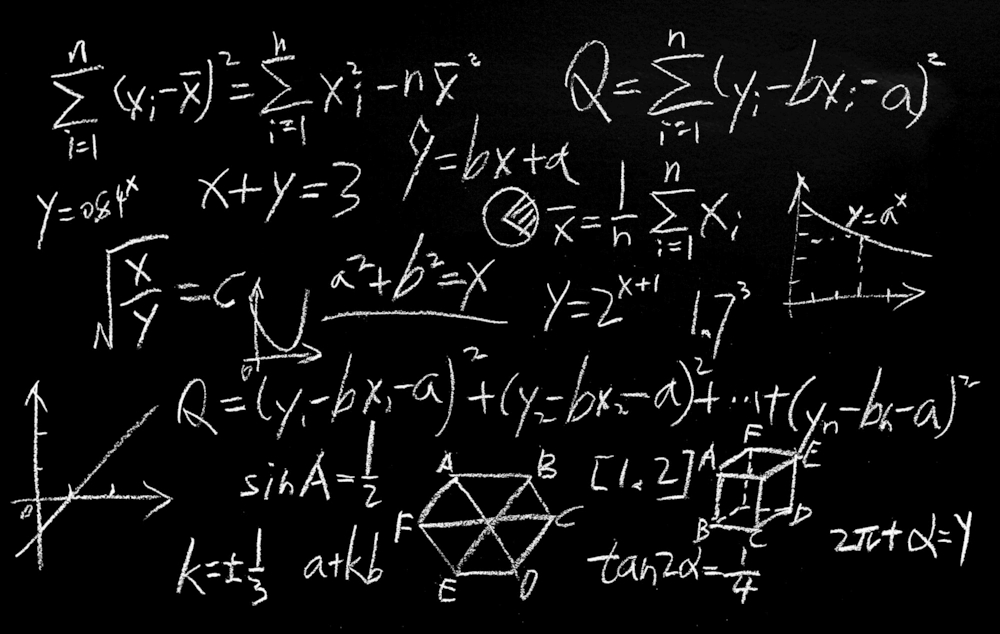
\includegraphics[scale=1.2,angle=45]{math.jpg}
	\caption{matho equations}
	\label{fig:mathequation}
\end{figure}

\pagebreak
\section{Bibliography}

\begin{thebibliography}{}

\bibitem{DBHS1}
Alcosser, Howard.
''Diamond Bar High School.''
\textit{Internal Accessment: Mathmatical Exploration}.
Web, 27 May 2018. 
\end{thebibliography}




\end{document}